\begin{activity}{Rock Fabric \& Mixing Laws}

\section*{Purpose}

This activity develops visual intuition for how rock texture and fabric determine which mixing law is appropriate for estimating bulk physical properties. By classifying a series of rock photographs at different scales, you will connect the geometry of a material to the mathematical model best suited to describe its effective properties.

\section*{Learning Outcomes}

By the end of this activity, you should be able to:
\begin{itemize}
  \item Identify the fabric or geometry of a rock from a photograph and classify it as random granular, layered parallel, or layered in series.
  \item Select the appropriate mixing law (arithmetic, geometric, or harmonic) for density and thermal conductivity given a rock's geometry.
  \item Determine whether a material is isotropic or anisotropic at a given scale of observation.
\end{itemize}

\section*{Background}

Mixing relationships are mathematical methods that we use to approximate the physical behavior of an rock from its constituent mineralogy and porosity.  These relationships can sometimes be derived from first principals---as we'll show for harmonic means and thermal conductivity later in the course---though more often they are empirical approximations that capture the messiness of the world.

Physical properties can be divided into two broad classes.

\textbf{Bulk properties} depend primarily on the amount of each constituent material present and are relatively insensitive to how those materials are arranged. Examples include density ($\rho$) and specific heat capacity ($C_P$). These properties are generally estimated using volume-weighted arithmetic averages.

\medskip

\textbf{Geometry-controlled properties} depend not only on the constituent materials but also on how they are distributed and connected. Examples include thermal conductivity ($k$), electrical conductivity ($\sigma$), and many elastic properties (bulk and shear moduli). For these properties, the appropriate mixing relationship depends on the geometry and orientation of the materials.

\begin{table}[h]
  \centering
  \caption{Guidelines for selecting mixing relationships.}
  \renewcommand{\arraystretch}{1.3}
  \begin{tabularx}{\textwidth}{@{}YlYY@{}}
    \toprule
    \textbf{Geometry / Fabric} &
    \textbf{Density} &
    \textbf{Conductivity} &
    \textbf{Elastic Moduli} \\
    \midrule

    Random granular mixture &
    Arithmetic &
    Geometric &
    Voigt--Reuss--Hill \\

    Layered, parallel to transport &
    Arithmetic &
    Arithmetic &
    Direction-dependent \\

    Layered, perpendicular to transport &
    Arithmetic &
    Harmonic &
    Direction-dependent \\

    Strongly fractured or porous material &
    Arithmetic &
    Depends on connectivity; often harmonic-like &
    Depends on fracture geometry and filling \\
    \bottomrule
  \end{tabularx}
\end{table}

\section*{Instructions:}  

Open the slide deck (\verb+isotropy_anisotropy.ppt+) on \LMS\ course website.  The pictures of rocks range from micrographs to aerial photos.  For each photo, ask:
\begin{quote}
  If this were a gravity survey, would the distinction between individual minerals matter?

  If this were a conductivity problem, would connectivity matter?

  Consider how your interpretation might \textbf{change at a different scale}.  
\end{quote}

For each photo fill in your responses that:  
\begin{itemize}
    \item Identify the \textbf{fabric/geometry}.  
    \item Identify the \textbf{approximate scale} of the photo.
    \item Select an appropriate \textbf{mixing law for density} ($\rho$).  
    \item Select an appropriate \textbf{mixing law for thermal conductivity} ($k$).  
    \item State whether the material is \textbf{isotropic or anisotropic} at this scale.  
\end{itemize}

\vspace{1em}

% ---------------------------------------------------------------
% RESPONSE GRID
% ---------------------------------------------------------------
{\small
\begin{tabularx}{\textwidth}{@{}|c|Y|Y|Y|Y|Y|@{}}
  \toprule
  & & \textbf{Scale} & \multicolumn{2}{c|}{\textbf{Mixing Law}} & \\
  & & & \multicolumn{2}{c|}{(\textbf{A})rithmetic, (\textbf{G})eometric, (\textbf{H})armonic} & \\
  \textbf{Photo} &
  \textbf{Description} &
  \textbf{Micro / Macro / Meso} &
  \textbf{Density} &
  \textbf{Thermal Conductivity} &
  \textbf{(I)sotropic / (A)nisotropic} \\
  \midrule
  \textbf{Example} & uniform porous sandstone & Meso & A & G & I \\
  \midrule
  \textbf{\#1}\rule{0pt}{2em} & & & & & \\
  \midrule
  \textbf{\#2}\rule{0pt}{2em} & & & & & \\
  \midrule
  \textbf{\#3}\rule{0pt}{2em} & & & & & \\
  \midrule
  \textbf{\#4}\rule{0pt}{2em} & & & & & \\
  \midrule
  \textbf{\#5}\rule{0pt}{2em} & & & & & \\
  \midrule
  \textbf{\#6}\rule{0pt}{2em} & & & & & \\
  \midrule
  \textbf{\#7}\rule{0pt}{2em} & & & & & \\
  \midrule
  \textbf{\#8}\rule{0pt}{2em} & & & & & \\
  \midrule
  \textbf{\#9}\rule{0pt}{2em} & & & & & \\
  \midrule
  \textbf{\#10}\rule{0pt}{2em} & & & & & \\
  \midrule
  \textbf{\#11}\rule{0pt}{2em} & & & & & \\
  \midrule
  \textbf{\#12}\rule{0pt}{2em} & & & & & \\
  \midrule
  \textbf{\#13}\rule{0pt}{2em} & & & & & \\
  \midrule
  \textbf{\#14}\rule{0pt}{2em} & & & & & \\
  \midrule
  \textbf{\#15}\rule{0pt}{2em} & & & & & \\
  \bottomrule
\end{tabularx}
}

\bigskip

\section*{Key Ideas}
For bulk rock properties, an arithmetic mean is always used to compute the effective property estimate.

For pathway sensitive properties, 
\begin{figure}[h]
\centering

\begin{minipage}{0.30\textwidth}
  \centering
  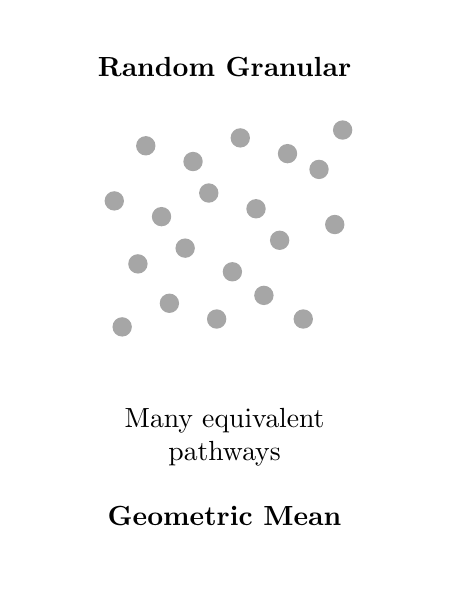
\begin{tikzpicture}
    \path[use as bounding box] (-1,-2) rectangle (4,5);

    % Title
    \node[font=\bfseries] at (1.5,4.5) {Random Granular};

    % Figure
    \foreach \x/\y in {
    0.2/0.2,0.8/0.5,1.4/0.3,2.0/0.6,3/2.7,
    0.4/1.0,1.0/1.2,1.6/0.9,2.2/1.3,2.7/2.2,
    0.1/1.8,0.7/1.6,1.3/1.9,1.9/1.7,2.9/1.5,
    0.5/2.5,1.1/2.3,1.7/2.6,2.3/2.4,2.5/0.3}
    {
      \fill[gray!70] (\x,\y+1) circle (3.5pt);
    }

    % Description
    \node[align=center] at (1.5,-0.2)
        {Many equivalent\\pathways};

    % Mean
    \node[font=\bfseries] at (1.5,-1.2)
        {Geometric Mean};
  \end{tikzpicture}
\end{minipage}
\hfill
\begin{minipage}{0.30\textwidth}
  \centering
  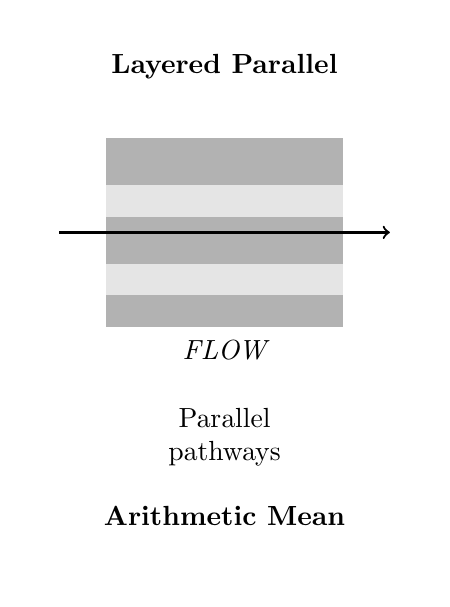
\begin{tikzpicture}
    \path[use as bounding box] (-1,-2) rectangle (4,5);
    % Title
    \node[font=\bfseries] at (1.5,4.5) {Layered Parallel};

    % Figure
    \fill[gray!60] (0,1.2) rectangle (3,1.6);
    \fill[gray!20] (0,1.6) rectangle (3,2.0);
    \fill[gray!60] (0,2.0) rectangle (3,2.6);
    \fill[gray!20] (0,2.6) rectangle (3,3.0);
    \fill[gray!60] (0,3.0) rectangle (3,3.6);

    \draw[->,thick] (-0.6,2.4) -- (3.6,2.4);
    \node[font=\itshape] at (1.5,0.9) {FLOW};

    % Description
    \node[align=center] at (1.5,-0.2)
        {Parallel\\pathways};

    % Mean
    \node[font=\bfseries] at (1.5,-1.2)
        {Arithmetic Mean};
  \end{tikzpicture}
\end{minipage}
\hfill
\begin{minipage}{0.30\textwidth}
  \centering
  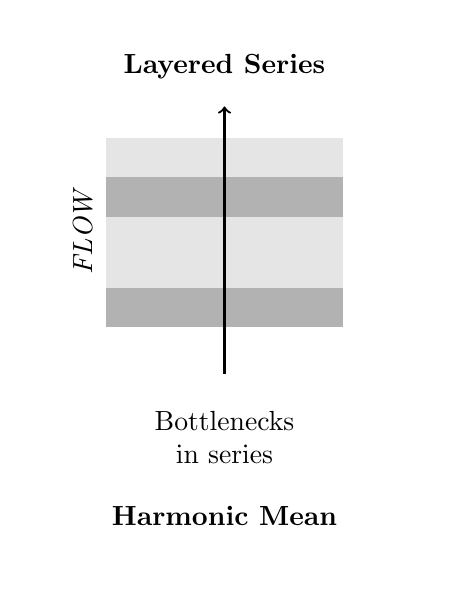
\begin{tikzpicture}
    \path[use as bounding box] (-1,-2) rectangle (4,5);
    % Title
    \node[font=\bfseries] at (1.5,4.5) {Layered Series};

    % Figure
    \fill[gray!60] (0,1.2) rectangle (3,1.7);
    \fill[gray!20] (0,1.7) rectangle (3,2.0);
    \fill[gray!20] (0,2.0) rectangle (3,2.6);
    \fill[gray!60] (0,2.6) rectangle (3,3.1);
    \fill[gray!20] (0,3.1) rectangle (3,3.6);

    \draw[->,thick] (1.5,0.6) -- (1.5,4.0);
    \node[rotate=90,font=\itshape] at (-0.3,2.4) {FLOW};

    % Description
    \node[align=center] at (1.5,-0.2)
        {Bottlenecks\\in series};

    % Mean
    \node[font=\bfseries] at (1.5,-1.2)
        {Harmonic Mean};
  \end{tikzpicture}
\end{minipage}

\caption{Conceptual relationship between fabric, transport geometry, and appropriate mixing relationship.}
\end{figure}

\vfill
\end{activity}